\begin{frame}[t]
	\frametitle{Model problem with known exact solution}\begin{center}
	\eqnboxc[.9\textwidth]{
		2-group neutron diffusion problem with source $Q^g$, B.C.:
		\shorten{-.7em}{-1.2em}
		\begin{align*}
			\fl^g &= 0\quad\ \on{\fl}\\
			-\bn\cdot D^g\nabla \fl^g &= 0\quad\ \on{sym}\\
			 \bn\cdot D^g\nabla \fl^g + \gamma^g\fl^g &= 0\quad\ \on{\gamma}
		\end{align*}
		\lengthen
	}
	\eqnboxc[.9\textwidth]{
		Exact solution\\[.4em]\hrule
		\begin{align*}
			\fl^1(x,y) &= \mathrm{e}^{-4 x^2} \left(\frac{y}{2}-\frac{y^2}{4}\right)\\
			\fl^2(x,y) &= \frac{1}{10} (\sin^2(4 \pi x) \sin^2(4 \pi y)+1) \fl^1(x,y)
		\end{align*}
		\structure{$\Ra$} \alert{$\gamma^1 = \gamma^2 = 8,\quad Q^1(x,y),\ Q^2(x,y)$}
	}	
	\end{center}
\end{frame}

\begin{frame}[c]
	\frametitle{Solution by Mathematica: \alt<1>{$\fl^1,\,\fl^2$}{$Q^1,\,Q^2$}}
	\begin{tikzpicture}[overlay]
		\node<1>[below=-3.3cm] at (current page.center) [inner sep=0pt, draw=structure, line width=2mm] {
			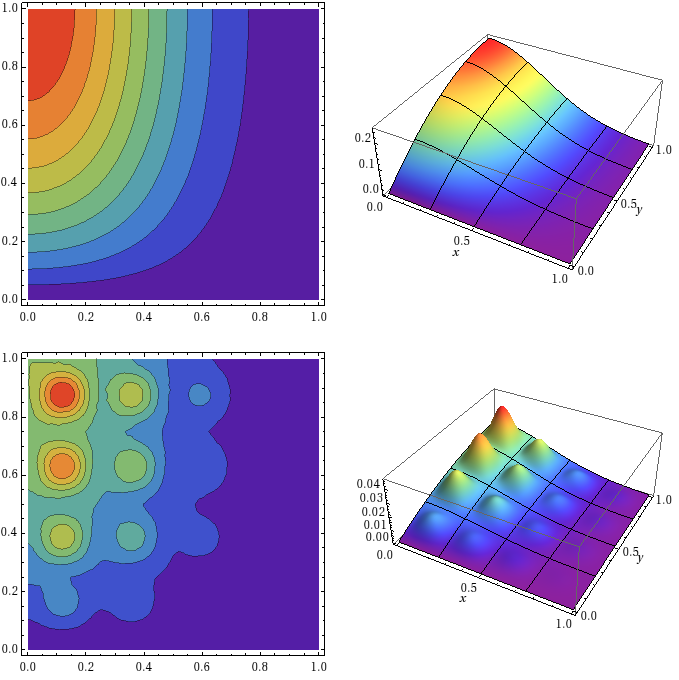
\includegraphics[scale=.3]{images/exact/F}
		};
		\node<2>[below=-3.3cm] at (current page.center) [inner sep=0pt, draw=structure, line width=2mm] {
			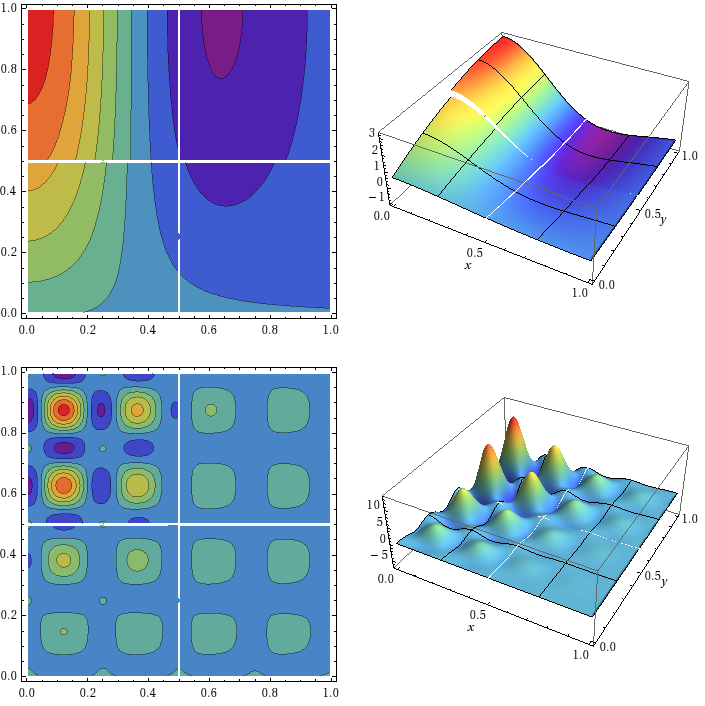
\includegraphics[scale=.3]{images/exact/Q}
		};
	\end{tikzpicture}
\end{frame}

\begin{frame}[c]
	\frametitle{Solution by Hermes \\[-.25em]{\scriptsize for each group (left to right), solution and difference from the exact solution}}
		\begin{tikzpicture}[overlay]
		\node[above left=-.6cm and .025cm of current page.center] (f1) [inner sep=0pt] {
			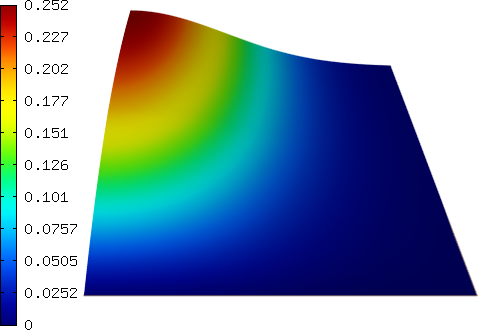
\includegraphics[height=3.5cm]{images/312121/F1}
		};
		\node[right=.25cm] at (f1.east) [inner sep=0pt] {
			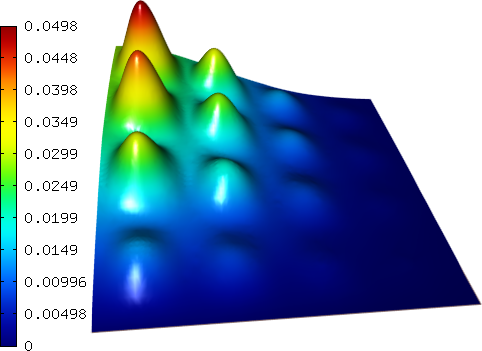
\includegraphics[height=3.5cm]{images/312121/F2}
		};
		\node[below=.25cm of f1.south, inner sep=0pt] (err1) {
			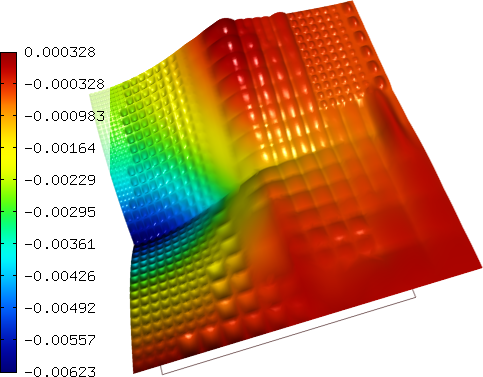
\includegraphics[height=3.5cm]{images/312121/err1}
		};
		\node[right=.65cm of err1.east, inner sep=0pt] {
			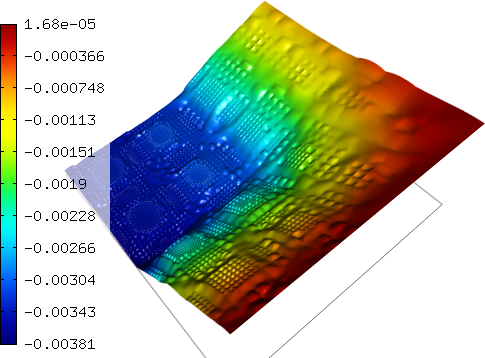
\includegraphics[height=3.5cm]{images/312121/err2}
		};
	\end{tikzpicture}
\end{frame}

\begin{frame}[c]
	\frametitle{Final grids for each group}
		\begin{tikzpicture}[overlay]
		\node[left=.25cm  of current page.center] (f1) [inner sep=0pt] {
			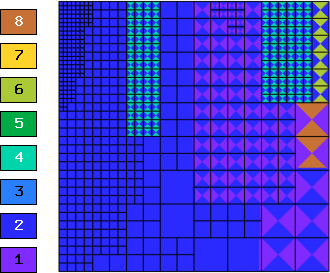
\includegraphics[width=.5\textwidth]{images/312121/grid1}
		};
		\node[right=.5cm] at (f1.east) [inner sep=0pt] {
			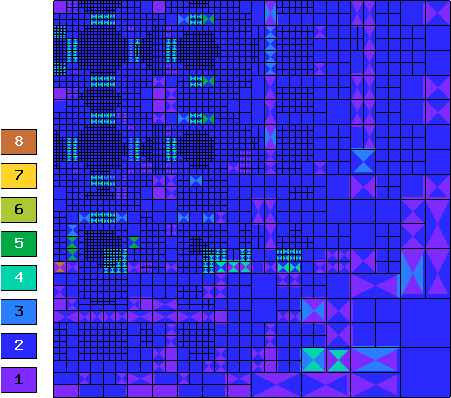
\includegraphics[width=.5\textwidth]{images/312121/grid2}
		};
	\end{tikzpicture}
\end{frame}

\begin{frame}[c]
	\frametitle{Convergence graphs}
	\begin{tikzpicture}[gnuplot]
		\only<1>{%% \begin{tikzpicture}[gnuplot]
%% generated with GNUPLOT 4.4p0 (Lua 5.1.4; terminal rev. 97, script rev. 96a)
%% Út 8. červen 2010, 18:51:53 CEST
\gpcolor{gp lt color axes}
\gpsetlinetype{gp lt axes}
\gpsetlinewidth{1.00}
\draw[gp path] (2.056,0.985)--(9.039,0.985);
\gpcolor{gp lt color border}
\gpsetlinetype{gp lt border}
\draw[gp path] (2.056,0.985)--(2.236,0.985);
\draw[gp path] (9.039,0.985)--(8.859,0.985);
\node[gp node right] at (1.872,0.985) { 0.001};
\draw[gp path] (2.056,1.261)--(2.146,1.261);
\draw[gp path] (9.039,1.261)--(8.949,1.261);
\draw[gp path] (2.056,1.627)--(2.146,1.627);
\draw[gp path] (9.039,1.627)--(8.949,1.627);
\draw[gp path] (2.056,1.814)--(2.146,1.814);
\draw[gp path] (9.039,1.814)--(8.949,1.814);
\gpcolor{gp lt color axes}
\gpsetlinetype{gp lt axes}
\draw[gp path] (2.056,1.903)--(9.039,1.903);
\gpcolor{gp lt color border}
\gpsetlinetype{gp lt border}
\draw[gp path] (2.056,1.903)--(2.236,1.903);
\draw[gp path] (9.039,1.903)--(8.859,1.903);
\node[gp node right] at (1.872,1.903) { 0.01};
\draw[gp path] (2.056,2.179)--(2.146,2.179);
\draw[gp path] (9.039,2.179)--(8.949,2.179);
\draw[gp path] (2.056,2.545)--(2.146,2.545);
\draw[gp path] (9.039,2.545)--(8.949,2.545);
\draw[gp path] (2.056,2.732)--(2.146,2.732);
\draw[gp path] (9.039,2.732)--(8.949,2.732);
\gpcolor{gp lt color axes}
\gpsetlinetype{gp lt axes}
\draw[gp path] (2.056,2.821)--(9.039,2.821);
\gpcolor{gp lt color border}
\gpsetlinetype{gp lt border}
\draw[gp path] (2.056,2.821)--(2.236,2.821);
\draw[gp path] (9.039,2.821)--(8.859,2.821);
\node[gp node right] at (1.872,2.821) { 0.1};
\draw[gp path] (2.056,3.097)--(2.146,3.097);
\draw[gp path] (9.039,3.097)--(8.949,3.097);
\draw[gp path] (2.056,3.463)--(2.146,3.463);
\draw[gp path] (9.039,3.463)--(8.949,3.463);
\draw[gp path] (2.056,3.650)--(2.146,3.650);
\draw[gp path] (9.039,3.650)--(8.949,3.650);
\gpcolor{gp lt color axes}
\gpsetlinetype{gp lt axes}
\draw[gp path] (2.056,3.739)--(9.039,3.739);
\gpcolor{gp lt color border}
\gpsetlinetype{gp lt border}
\draw[gp path] (2.056,3.739)--(2.236,3.739);
\draw[gp path] (9.039,3.739)--(8.859,3.739);
\node[gp node right] at (1.872,3.739) { 1};
\draw[gp path] (2.056,4.015)--(2.146,4.015);
\draw[gp path] (9.039,4.015)--(8.949,4.015);
\draw[gp path] (2.056,4.381)--(2.146,4.381);
\draw[gp path] (9.039,4.381)--(8.949,4.381);
\draw[gp path] (2.056,4.568)--(2.146,4.568);
\draw[gp path] (9.039,4.568)--(8.949,4.568);
\gpcolor{gp lt color axes}
\gpsetlinetype{gp lt axes}
\draw[gp path] (2.056,4.657)--(9.039,4.657);
\gpcolor{gp lt color border}
\gpsetlinetype{gp lt border}
\draw[gp path] (2.056,4.657)--(2.236,4.657);
\draw[gp path] (9.039,4.657)--(8.859,4.657);
\node[gp node right] at (1.872,4.657) { 10};
\draw[gp path] (2.056,4.933)--(2.146,4.933);
\draw[gp path] (9.039,4.933)--(8.949,4.933);
\draw[gp path] (2.056,5.299)--(2.146,5.299);
\draw[gp path] (9.039,5.299)--(8.949,5.299);
\draw[gp path] (2.056,5.486)--(2.146,5.486);
\draw[gp path] (9.039,5.486)--(8.949,5.486);
\gpcolor{gp lt color axes}
\gpsetlinetype{gp lt axes}
\draw[gp path] (2.056,5.575)--(9.039,5.575);
\gpcolor{gp lt color border}
\gpsetlinetype{gp lt border}
\draw[gp path] (2.056,5.575)--(2.236,5.575);
\draw[gp path] (9.039,5.575)--(8.859,5.575);
\node[gp node right] at (1.872,5.575) { 100};
\gpcolor{gp lt color axes}
\gpsetlinetype{gp lt axes}
\draw[gp path] (2.056,0.985)--(2.056,5.575);
\gpcolor{gp lt color border}
\gpsetlinetype{gp lt border}
\draw[gp path] (2.056,0.985)--(2.056,1.165);
\draw[gp path] (2.056,5.575)--(2.056,5.395);
\node[gp node center] at (2.056,0.677) { 100};
\draw[gp path] (2.757,0.985)--(2.757,1.075);
\draw[gp path] (2.757,5.575)--(2.757,5.485);
\draw[gp path] (3.167,0.985)--(3.167,1.075);
\draw[gp path] (3.167,5.575)--(3.167,5.485);
\draw[gp path] (3.457,0.985)--(3.457,1.075);
\draw[gp path] (3.457,5.575)--(3.457,5.485);
\draw[gp path] (3.683,0.985)--(3.683,1.075);
\draw[gp path] (3.683,5.575)--(3.683,5.485);
\draw[gp path] (3.867,0.985)--(3.867,1.075);
\draw[gp path] (3.867,5.575)--(3.867,5.485);
\draw[gp path] (4.023,0.985)--(4.023,1.075);
\draw[gp path] (4.023,5.575)--(4.023,5.485);
\draw[gp path] (4.158,0.985)--(4.158,1.075);
\draw[gp path] (4.158,5.575)--(4.158,5.485);
\draw[gp path] (4.277,0.985)--(4.277,1.075);
\draw[gp path] (4.277,5.575)--(4.277,5.485);
\gpcolor{gp lt color axes}
\gpsetlinetype{gp lt axes}
\draw[gp path] (4.384,0.985)--(4.384,5.575);
\gpcolor{gp lt color border}
\gpsetlinetype{gp lt border}
\draw[gp path] (4.384,0.985)--(4.384,1.165);
\draw[gp path] (4.384,5.575)--(4.384,5.395);
\node[gp node center] at (4.384,0.677) { 1000};
\draw[gp path] (5.084,0.985)--(5.084,1.075);
\draw[gp path] (5.084,5.575)--(5.084,5.485);
\draw[gp path] (5.494,0.985)--(5.494,1.075);
\draw[gp path] (5.494,5.575)--(5.494,5.485);
\draw[gp path] (5.785,0.985)--(5.785,1.075);
\draw[gp path] (5.785,5.575)--(5.785,5.485);
\draw[gp path] (6.011,0.985)--(6.011,1.075);
\draw[gp path] (6.011,5.575)--(6.011,5.485);
\draw[gp path] (6.195,0.985)--(6.195,1.075);
\draw[gp path] (6.195,5.575)--(6.195,5.485);
\draw[gp path] (6.351,0.985)--(6.351,1.075);
\draw[gp path] (6.351,5.575)--(6.351,5.485);
\draw[gp path] (6.486,0.985)--(6.486,1.075);
\draw[gp path] (6.486,5.575)--(6.486,5.485);
\draw[gp path] (6.605,0.985)--(6.605,1.075);
\draw[gp path] (6.605,5.575)--(6.605,5.485);
\gpcolor{gp lt color axes}
\gpsetlinetype{gp lt axes}
\draw[gp path] (6.711,0.985)--(6.711,4.779);
\draw[gp path] (6.711,5.395)--(6.711,5.575);
\gpcolor{gp lt color border}
\gpsetlinetype{gp lt border}
\draw[gp path] (6.711,0.985)--(6.711,1.165);
\draw[gp path] (6.711,5.575)--(6.711,5.395);
\node[gp node center] at (6.711,0.677) { 10000};
\draw[gp path] (7.412,0.985)--(7.412,1.075);
\draw[gp path] (7.412,5.575)--(7.412,5.485);
\draw[gp path] (7.822,0.985)--(7.822,1.075);
\draw[gp path] (7.822,5.575)--(7.822,5.485);
\draw[gp path] (8.113,0.985)--(8.113,1.075);
\draw[gp path] (8.113,5.575)--(8.113,5.485);
\draw[gp path] (8.338,0.985)--(8.338,1.075);
\draw[gp path] (8.338,5.575)--(8.338,5.485);
\draw[gp path] (8.523,0.985)--(8.523,1.075);
\draw[gp path] (8.523,5.575)--(8.523,5.485);
\draw[gp path] (8.678,0.985)--(8.678,1.075);
\draw[gp path] (8.678,5.575)--(8.678,5.485);
\draw[gp path] (8.813,0.985)--(8.813,1.075);
\draw[gp path] (8.813,5.575)--(8.813,5.485);
\draw[gp path] (8.932,0.985)--(8.932,1.075);
\draw[gp path] (8.932,5.575)--(8.932,5.485);
\gpcolor{gp lt color axes}
\gpsetlinetype{gp lt axes}
\draw[gp path] (9.039,0.985)--(9.039,5.575);
\gpcolor{gp lt color border}
\gpsetlinetype{gp lt border}
\draw[gp path] (9.039,0.985)--(9.039,1.165);
\draw[gp path] (9.039,5.575)--(9.039,5.395);
\node[gp node center] at (9.039,0.677) { 100000};
\draw[gp path] (2.056,5.575)--(2.056,0.985)--(9.039,0.985)--(9.039,5.575)--cycle;
\node[gp node center,rotate=-270] at (0.430,3.280) {Error [\%]};
\node[gp node center] at (5.547,0.215) {Degrees of freedom};
\node[gp node center] at (5.547,6.037) {Error convergence};
\node[gp node right] at (7.571,5.241) {exact error};
\gpcolor{gp lt color 2}
\gpsetlinetype{gp lt plot 0}
\gpsetlinewidth{2.00}
\draw[gp path] (7.755,5.241)--(8.671,5.241);
\draw[gp path] (2.418,5.551)--(2.811,5.478)--(2.830,5.472)--(2.937,5.443)--(2.966,5.438)%
  --(3.392,5.378)--(3.408,5.374)--(3.507,5.364)--(3.936,5.105)--(3.944,5.053)--(3.953,5.011)%
  --(4.114,4.971)--(4.500,4.860)--(4.509,4.845)--(4.728,4.755)--(4.740,4.743)--(5.165,4.677)%
  --(5.368,4.668)--(5.710,4.559)--(5.717,4.545)--(5.996,4.522)--(6.029,4.498)--(6.048,4.496)%
  --(6.161,4.493)--(6.420,4.495)--(6.528,4.488)--(6.550,4.489)--(6.603,4.490)--(6.687,4.488)%
  --(6.915,4.490)--(7.049,4.495)--(7.224,4.497);
\gpsetpointsize{4.00}
\gppoint{gp mark 6}{(2.418,5.551)}
\gppoint{gp mark 6}{(2.811,5.478)}
\gppoint{gp mark 6}{(2.830,5.472)}
\gppoint{gp mark 6}{(2.937,5.443)}
\gppoint{gp mark 6}{(2.966,5.438)}
\gppoint{gp mark 6}{(3.392,5.378)}
\gppoint{gp mark 6}{(3.408,5.374)}
\gppoint{gp mark 6}{(3.507,5.364)}
\gppoint{gp mark 6}{(3.936,5.105)}
\gppoint{gp mark 6}{(3.944,5.053)}
\gppoint{gp mark 6}{(3.953,5.011)}
\gppoint{gp mark 6}{(4.114,4.971)}
\gppoint{gp mark 6}{(4.500,4.860)}
\gppoint{gp mark 6}{(4.509,4.845)}
\gppoint{gp mark 6}{(4.728,4.755)}
\gppoint{gp mark 6}{(4.740,4.743)}
\gppoint{gp mark 6}{(5.165,4.677)}
\gppoint{gp mark 6}{(5.368,4.668)}
\gppoint{gp mark 6}{(5.710,4.559)}
\gppoint{gp mark 6}{(5.717,4.545)}
\gppoint{gp mark 6}{(5.996,4.522)}
\gppoint{gp mark 6}{(6.029,4.498)}
\gppoint{gp mark 6}{(6.048,4.496)}
\gppoint{gp mark 6}{(6.161,4.493)}
\gppoint{gp mark 6}{(6.420,4.495)}
\gppoint{gp mark 6}{(6.528,4.488)}
\gppoint{gp mark 6}{(6.550,4.489)}
\gppoint{gp mark 6}{(6.603,4.490)}
\gppoint{gp mark 6}{(6.687,4.488)}
\gppoint{gp mark 6}{(6.915,4.490)}
\gppoint{gp mark 6}{(7.049,4.495)}
\gppoint{gp mark 6}{(7.224,4.497)}
\gppoint{gp mark 6}{(8.213,5.241)}
\gpcolor{gp lt color border}
\node[gp node right] at (7.571,4.933) {est. error };
\gpcolor{gp lt color 0}
\draw[gp path] (7.755,4.933)--(8.671,4.933);
\draw[gp path] (2.418,3.461)--(2.811,3.612)--(2.830,3.478)--(2.937,3.399)--(2.966,3.336)%
  --(3.392,3.271)--(3.408,3.216)--(3.507,3.158)--(3.936,3.216)--(3.944,3.098)--(3.953,3.041)%
  --(4.114,2.948)--(4.500,2.842)--(4.509,2.825)--(4.728,2.700)--(4.740,2.690)--(5.165,2.514)%
  --(5.368,2.440)--(5.710,2.320)--(5.717,2.313)--(5.996,2.201)--(6.029,2.190)--(6.048,2.178)%
  --(6.161,2.125)--(6.420,2.033)--(6.528,1.995)--(6.550,1.987)--(6.603,1.966)--(6.687,1.934)%
  --(6.915,1.846)--(7.049,1.791)--(7.224,1.717);
\gppoint{gp mark 4}{(2.418,3.461)}
\gppoint{gp mark 4}{(2.811,3.612)}
\gppoint{gp mark 4}{(2.830,3.478)}
\gppoint{gp mark 4}{(2.937,3.399)}
\gppoint{gp mark 4}{(2.966,3.336)}
\gppoint{gp mark 4}{(3.392,3.271)}
\gppoint{gp mark 4}{(3.408,3.216)}
\gppoint{gp mark 4}{(3.507,3.158)}
\gppoint{gp mark 4}{(3.936,3.216)}
\gppoint{gp mark 4}{(3.944,3.098)}
\gppoint{gp mark 4}{(3.953,3.041)}
\gppoint{gp mark 4}{(4.114,2.948)}
\gppoint{gp mark 4}{(4.500,2.842)}
\gppoint{gp mark 4}{(4.509,2.825)}
\gppoint{gp mark 4}{(4.728,2.700)}
\gppoint{gp mark 4}{(4.740,2.690)}
\gppoint{gp mark 4}{(5.165,2.514)}
\gppoint{gp mark 4}{(5.368,2.440)}
\gppoint{gp mark 4}{(5.710,2.320)}
\gppoint{gp mark 4}{(5.717,2.313)}
\gppoint{gp mark 4}{(5.996,2.201)}
\gppoint{gp mark 4}{(6.029,2.190)}
\gppoint{gp mark 4}{(6.048,2.178)}
\gppoint{gp mark 4}{(6.161,2.125)}
\gppoint{gp mark 4}{(6.420,2.033)}
\gppoint{gp mark 4}{(6.528,1.995)}
\gppoint{gp mark 4}{(6.550,1.987)}
\gppoint{gp mark 4}{(6.603,1.966)}
\gppoint{gp mark 4}{(6.687,1.934)}
\gppoint{gp mark 4}{(6.915,1.846)}
\gppoint{gp mark 4}{(7.049,1.791)}
\gppoint{gp mark 4}{(7.224,1.717)}
\gppoint{gp mark 4}{(8.213,4.933)}
\gpcolor{gp lt color border}
\gpsetlinetype{gp lt border}
\gpsetlinewidth{1.00}
\draw[gp path] (2.056,5.575)--(2.056,0.985)--(9.039,0.985)--(9.039,5.575)--cycle;
%% coordinates of the plot area
\gpdefrectangularnode{gp plot 1}{\pgfpoint{2.056cm}{0.985cm}}{\pgfpoint{9.039cm}{5.575cm}}
%% \end{tikzpicture}
%% gnuplot variables
}
		\only<2>{%% \begin{tikzpicture}[gnuplot]
%% generated with GNUPLOT 4.4p0 (Lua 5.1.4; terminal rev. 97, script rev. 96a)
%% Út 8. červen 2010, 18:51:53 CEST
\gpcolor{gp lt color axes}
\gpsetlinetype{gp lt axes}
\gpsetlinewidth{1.00}
\draw[gp path] (2.056,0.985)--(9.039,0.985);
\gpcolor{gp lt color border}
\gpsetlinetype{gp lt border}
\draw[gp path] (2.056,0.985)--(2.236,0.985);
\draw[gp path] (9.039,0.985)--(8.859,0.985);
\node[gp node right] at (1.872,0.985) { 0.001};
\draw[gp path] (2.056,1.261)--(2.146,1.261);
\draw[gp path] (9.039,1.261)--(8.949,1.261);
\draw[gp path] (2.056,1.627)--(2.146,1.627);
\draw[gp path] (9.039,1.627)--(8.949,1.627);
\draw[gp path] (2.056,1.814)--(2.146,1.814);
\draw[gp path] (9.039,1.814)--(8.949,1.814);
\gpcolor{gp lt color axes}
\gpsetlinetype{gp lt axes}
\draw[gp path] (2.056,1.903)--(9.039,1.903);
\gpcolor{gp lt color border}
\gpsetlinetype{gp lt border}
\draw[gp path] (2.056,1.903)--(2.236,1.903);
\draw[gp path] (9.039,1.903)--(8.859,1.903);
\node[gp node right] at (1.872,1.903) { 0.01};
\draw[gp path] (2.056,2.179)--(2.146,2.179);
\draw[gp path] (9.039,2.179)--(8.949,2.179);
\draw[gp path] (2.056,2.545)--(2.146,2.545);
\draw[gp path] (9.039,2.545)--(8.949,2.545);
\draw[gp path] (2.056,2.732)--(2.146,2.732);
\draw[gp path] (9.039,2.732)--(8.949,2.732);
\gpcolor{gp lt color axes}
\gpsetlinetype{gp lt axes}
\draw[gp path] (2.056,2.821)--(9.039,2.821);
\gpcolor{gp lt color border}
\gpsetlinetype{gp lt border}
\draw[gp path] (2.056,2.821)--(2.236,2.821);
\draw[gp path] (9.039,2.821)--(8.859,2.821);
\node[gp node right] at (1.872,2.821) { 0.1};
\draw[gp path] (2.056,3.097)--(2.146,3.097);
\draw[gp path] (9.039,3.097)--(8.949,3.097);
\draw[gp path] (2.056,3.463)--(2.146,3.463);
\draw[gp path] (9.039,3.463)--(8.949,3.463);
\draw[gp path] (2.056,3.650)--(2.146,3.650);
\draw[gp path] (9.039,3.650)--(8.949,3.650);
\gpcolor{gp lt color axes}
\gpsetlinetype{gp lt axes}
\draw[gp path] (2.056,3.739)--(9.039,3.739);
\gpcolor{gp lt color border}
\gpsetlinetype{gp lt border}
\draw[gp path] (2.056,3.739)--(2.236,3.739);
\draw[gp path] (9.039,3.739)--(8.859,3.739);
\node[gp node right] at (1.872,3.739) { 1};
\draw[gp path] (2.056,4.015)--(2.146,4.015);
\draw[gp path] (9.039,4.015)--(8.949,4.015);
\draw[gp path] (2.056,4.381)--(2.146,4.381);
\draw[gp path] (9.039,4.381)--(8.949,4.381);
\draw[gp path] (2.056,4.568)--(2.146,4.568);
\draw[gp path] (9.039,4.568)--(8.949,4.568);
\gpcolor{gp lt color axes}
\gpsetlinetype{gp lt axes}
\draw[gp path] (2.056,4.657)--(9.039,4.657);
\gpcolor{gp lt color border}
\gpsetlinetype{gp lt border}
\draw[gp path] (2.056,4.657)--(2.236,4.657);
\draw[gp path] (9.039,4.657)--(8.859,4.657);
\node[gp node right] at (1.872,4.657) { 10};
\draw[gp path] (2.056,4.933)--(2.146,4.933);
\draw[gp path] (9.039,4.933)--(8.949,4.933);
\draw[gp path] (2.056,5.299)--(2.146,5.299);
\draw[gp path] (9.039,5.299)--(8.949,5.299);
\draw[gp path] (2.056,5.486)--(2.146,5.486);
\draw[gp path] (9.039,5.486)--(8.949,5.486);
\gpcolor{gp lt color axes}
\gpsetlinetype{gp lt axes}
\draw[gp path] (2.056,5.575)--(9.039,5.575);
\gpcolor{gp lt color border}
\gpsetlinetype{gp lt border}
\draw[gp path] (2.056,5.575)--(2.236,5.575);
\draw[gp path] (9.039,5.575)--(8.859,5.575);
\node[gp node right] at (1.872,5.575) { 100};
\gpcolor{gp lt color axes}
\gpsetlinetype{gp lt axes}
\draw[gp path] (2.056,0.985)--(2.056,5.575);
\gpcolor{gp lt color border}
\gpsetlinetype{gp lt border}
\draw[gp path] (2.056,0.985)--(2.056,1.165);
\draw[gp path] (2.056,5.575)--(2.056,5.395);
\node[gp node center] at (2.056,0.677) { 0.1};
\draw[gp path] (2.582,0.985)--(2.582,1.075);
\draw[gp path] (2.582,5.575)--(2.582,5.485);
\draw[gp path] (2.889,0.985)--(2.889,1.075);
\draw[gp path] (2.889,5.575)--(2.889,5.485);
\draw[gp path] (3.107,0.985)--(3.107,1.075);
\draw[gp path] (3.107,5.575)--(3.107,5.485);
\draw[gp path] (3.276,0.985)--(3.276,1.075);
\draw[gp path] (3.276,5.575)--(3.276,5.485);
\draw[gp path] (3.414,0.985)--(3.414,1.075);
\draw[gp path] (3.414,5.575)--(3.414,5.485);
\draw[gp path] (3.531,0.985)--(3.531,1.075);
\draw[gp path] (3.531,5.575)--(3.531,5.485);
\draw[gp path] (3.633,0.985)--(3.633,1.075);
\draw[gp path] (3.633,5.575)--(3.633,5.485);
\draw[gp path] (3.722,0.985)--(3.722,1.075);
\draw[gp path] (3.722,5.575)--(3.722,5.485);
\gpcolor{gp lt color axes}
\gpsetlinetype{gp lt axes}
\draw[gp path] (3.802,0.985)--(3.802,5.575);
\gpcolor{gp lt color border}
\gpsetlinetype{gp lt border}
\draw[gp path] (3.802,0.985)--(3.802,1.165);
\draw[gp path] (3.802,5.575)--(3.802,5.395);
\node[gp node center] at (3.802,0.677) { 1};
\draw[gp path] (4.327,0.985)--(4.327,1.075);
\draw[gp path] (4.327,5.575)--(4.327,5.485);
\draw[gp path] (4.635,0.985)--(4.635,1.075);
\draw[gp path] (4.635,5.575)--(4.635,5.485);
\draw[gp path] (4.853,0.985)--(4.853,1.075);
\draw[gp path] (4.853,5.575)--(4.853,5.485);
\draw[gp path] (5.022,0.985)--(5.022,1.075);
\draw[gp path] (5.022,5.575)--(5.022,5.485);
\draw[gp path] (5.160,0.985)--(5.160,1.075);
\draw[gp path] (5.160,5.575)--(5.160,5.485);
\draw[gp path] (5.277,0.985)--(5.277,1.075);
\draw[gp path] (5.277,5.575)--(5.277,5.485);
\draw[gp path] (5.378,0.985)--(5.378,1.075);
\draw[gp path] (5.378,5.575)--(5.378,5.485);
\draw[gp path] (5.468,0.985)--(5.468,1.075);
\draw[gp path] (5.468,5.575)--(5.468,5.485);
\gpcolor{gp lt color axes}
\gpsetlinetype{gp lt axes}
\draw[gp path] (5.548,0.985)--(5.548,4.779);
\draw[gp path] (5.548,5.395)--(5.548,5.575);
\gpcolor{gp lt color border}
\gpsetlinetype{gp lt border}
\draw[gp path] (5.548,0.985)--(5.548,1.165);
\draw[gp path] (5.548,5.575)--(5.548,5.395);
\node[gp node center] at (5.548,0.677) { 10};
\draw[gp path] (6.073,0.985)--(6.073,1.075);
\draw[gp path] (6.073,5.575)--(6.073,5.485);
\draw[gp path] (6.380,0.985)--(6.380,1.075);
\draw[gp path] (6.380,5.575)--(6.380,5.485);
\draw[gp path] (6.599,0.985)--(6.599,1.075);
\draw[gp path] (6.599,5.575)--(6.599,5.485);
\draw[gp path] (6.768,0.985)--(6.768,1.075);
\draw[gp path] (6.768,5.575)--(6.768,5.485);
\draw[gp path] (6.906,0.985)--(6.906,1.075);
\draw[gp path] (6.906,5.575)--(6.906,5.485);
\draw[gp path] (7.023,0.985)--(7.023,1.075);
\draw[gp path] (7.023,5.575)--(7.023,5.485);
\draw[gp path] (7.124,0.985)--(7.124,1.075);
\draw[gp path] (7.124,5.575)--(7.124,5.485);
\draw[gp path] (7.213,0.985)--(7.213,1.075);
\draw[gp path] (7.213,5.575)--(7.213,5.485);
\gpcolor{gp lt color axes}
\gpsetlinetype{gp lt axes}
\draw[gp path] (7.293,0.985)--(7.293,4.779);
\draw[gp path] (7.293,5.395)--(7.293,5.575);
\gpcolor{gp lt color border}
\gpsetlinetype{gp lt border}
\draw[gp path] (7.293,0.985)--(7.293,1.165);
\draw[gp path] (7.293,5.575)--(7.293,5.395);
\node[gp node center] at (7.293,0.677) { 100};
\draw[gp path] (7.819,0.985)--(7.819,1.075);
\draw[gp path] (7.819,5.575)--(7.819,5.485);
\draw[gp path] (8.126,0.985)--(8.126,1.075);
\draw[gp path] (8.126,5.575)--(8.126,5.485);
\draw[gp path] (8.344,0.985)--(8.344,1.075);
\draw[gp path] (8.344,5.575)--(8.344,5.485);
\draw[gp path] (8.513,0.985)--(8.513,1.075);
\draw[gp path] (8.513,5.575)--(8.513,5.485);
\draw[gp path] (8.652,0.985)--(8.652,1.075);
\draw[gp path] (8.652,5.575)--(8.652,5.485);
\draw[gp path] (8.769,0.985)--(8.769,1.075);
\draw[gp path] (8.769,5.575)--(8.769,5.485);
\draw[gp path] (8.870,0.985)--(8.870,1.075);
\draw[gp path] (8.870,5.575)--(8.870,5.485);
\draw[gp path] (8.959,0.985)--(8.959,1.075);
\draw[gp path] (8.959,5.575)--(8.959,5.485);
\gpcolor{gp lt color axes}
\gpsetlinetype{gp lt axes}
\draw[gp path] (9.039,0.985)--(9.039,5.575);
\gpcolor{gp lt color border}
\gpsetlinetype{gp lt border}
\draw[gp path] (9.039,0.985)--(9.039,1.165);
\draw[gp path] (9.039,5.575)--(9.039,5.395);
\node[gp node center] at (9.039,0.677) { 1000};
\draw[gp path] (2.056,5.575)--(2.056,0.985)--(9.039,0.985)--(9.039,5.575)--cycle;
\node[gp node center,rotate=-270] at (0.430,3.280) {Error [\%]};
\node[gp node center] at (5.547,0.215) {CPU time [s]};
\node[gp node center] at (5.547,6.037) {Error convergence};
\node[gp node right] at (7.571,5.241) {exact error};
\gpcolor{gp lt color 2}
\gpsetlinetype{gp lt plot 0}
\gpsetlinewidth{2.00}
\draw[gp path] (7.755,5.241)--(8.671,5.241);
\draw[gp path] (3.673,5.551)--(4.006,5.478)--(4.217,5.472)--(4.434,5.443)--(4.595,5.438)%
  --(4.801,5.378)--(4.950,5.374)--(5.096,5.364)--(5.293,5.105)--(5.437,5.053)--(5.556,5.011)%
  --(5.679,4.971)--(5.831,4.860)--(5.950,4.845)--(6.068,4.755)--(6.166,4.743)--(6.308,4.677)%
  --(6.447,4.668)--(6.605,4.559)--(6.731,4.545)--(6.879,4.522)--(7.000,4.498)--(7.104,4.496)%
  --(7.205,4.493)--(7.320,4.495)--(7.430,4.488)--(7.527,4.489)--(7.618,4.490)--(7.706,4.488)%
  --(7.808,4.490)--(7.908,4.495)--(8.010,4.497);
\gpsetpointsize{4.00}
\gppoint{gp mark 6}{(3.673,5.551)}
\gppoint{gp mark 6}{(4.006,5.478)}
\gppoint{gp mark 6}{(4.217,5.472)}
\gppoint{gp mark 6}{(4.434,5.443)}
\gppoint{gp mark 6}{(4.595,5.438)}
\gppoint{gp mark 6}{(4.801,5.378)}
\gppoint{gp mark 6}{(4.950,5.374)}
\gppoint{gp mark 6}{(5.096,5.364)}
\gppoint{gp mark 6}{(5.293,5.105)}
\gppoint{gp mark 6}{(5.437,5.053)}
\gppoint{gp mark 6}{(5.556,5.011)}
\gppoint{gp mark 6}{(5.679,4.971)}
\gppoint{gp mark 6}{(5.831,4.860)}
\gppoint{gp mark 6}{(5.950,4.845)}
\gppoint{gp mark 6}{(6.068,4.755)}
\gppoint{gp mark 6}{(6.166,4.743)}
\gppoint{gp mark 6}{(6.308,4.677)}
\gppoint{gp mark 6}{(6.447,4.668)}
\gppoint{gp mark 6}{(6.605,4.559)}
\gppoint{gp mark 6}{(6.731,4.545)}
\gppoint{gp mark 6}{(6.879,4.522)}
\gppoint{gp mark 6}{(7.000,4.498)}
\gppoint{gp mark 6}{(7.104,4.496)}
\gppoint{gp mark 6}{(7.205,4.493)}
\gppoint{gp mark 6}{(7.320,4.495)}
\gppoint{gp mark 6}{(7.430,4.488)}
\gppoint{gp mark 6}{(7.527,4.489)}
\gppoint{gp mark 6}{(7.618,4.490)}
\gppoint{gp mark 6}{(7.706,4.488)}
\gppoint{gp mark 6}{(7.808,4.490)}
\gppoint{gp mark 6}{(7.908,4.495)}
\gppoint{gp mark 6}{(8.010,4.497)}
\gppoint{gp mark 6}{(8.213,5.241)}
\gpcolor{gp lt color border}
\node[gp node right] at (7.571,4.933) {est. error };
\gpcolor{gp lt color 0}
\draw[gp path] (7.755,4.933)--(8.671,4.933);
\draw[gp path] (3.673,3.461)--(4.006,3.612)--(4.217,3.478)--(4.434,3.399)--(4.595,3.336)%
  --(4.801,3.271)--(4.950,3.216)--(5.096,3.158)--(5.293,3.216)--(5.437,3.098)--(5.556,3.041)%
  --(5.679,2.948)--(5.831,2.842)--(5.950,2.825)--(6.068,2.700)--(6.166,2.690)--(6.308,2.514)%
  --(6.447,2.440)--(6.605,2.320)--(6.731,2.313)--(6.879,2.201)--(7.000,2.190)--(7.104,2.178)%
  --(7.205,2.125)--(7.320,2.033)--(7.430,1.995)--(7.527,1.987)--(7.618,1.966)--(7.706,1.934)%
  --(7.808,1.846)--(7.908,1.791)--(8.010,1.717);
\gppoint{gp mark 4}{(3.673,3.461)}
\gppoint{gp mark 4}{(4.006,3.612)}
\gppoint{gp mark 4}{(4.217,3.478)}
\gppoint{gp mark 4}{(4.434,3.399)}
\gppoint{gp mark 4}{(4.595,3.336)}
\gppoint{gp mark 4}{(4.801,3.271)}
\gppoint{gp mark 4}{(4.950,3.216)}
\gppoint{gp mark 4}{(5.096,3.158)}
\gppoint{gp mark 4}{(5.293,3.216)}
\gppoint{gp mark 4}{(5.437,3.098)}
\gppoint{gp mark 4}{(5.556,3.041)}
\gppoint{gp mark 4}{(5.679,2.948)}
\gppoint{gp mark 4}{(5.831,2.842)}
\gppoint{gp mark 4}{(5.950,2.825)}
\gppoint{gp mark 4}{(6.068,2.700)}
\gppoint{gp mark 4}{(6.166,2.690)}
\gppoint{gp mark 4}{(6.308,2.514)}
\gppoint{gp mark 4}{(6.447,2.440)}
\gppoint{gp mark 4}{(6.605,2.320)}
\gppoint{gp mark 4}{(6.731,2.313)}
\gppoint{gp mark 4}{(6.879,2.201)}
\gppoint{gp mark 4}{(7.000,2.190)}
\gppoint{gp mark 4}{(7.104,2.178)}
\gppoint{gp mark 4}{(7.205,2.125)}
\gppoint{gp mark 4}{(7.320,2.033)}
\gppoint{gp mark 4}{(7.430,1.995)}
\gppoint{gp mark 4}{(7.527,1.987)}
\gppoint{gp mark 4}{(7.618,1.966)}
\gppoint{gp mark 4}{(7.706,1.934)}
\gppoint{gp mark 4}{(7.808,1.846)}
\gppoint{gp mark 4}{(7.908,1.791)}
\gppoint{gp mark 4}{(8.010,1.717)}
\gppoint{gp mark 4}{(8.213,4.933)}
\gpcolor{gp lt color border}
\gpsetlinetype{gp lt border}
\gpsetlinewidth{1.00}
\draw[gp path] (2.056,5.575)--(2.056,0.985)--(9.039,0.985)--(9.039,5.575)--cycle;
%% coordinates of the plot area
\gpdefrectangularnode{gp plot 1}{\pgfpoint{2.056cm}{0.985cm}}{\pgfpoint{9.039cm}{5.575cm}}
%% \end{tikzpicture}
%% gnuplot variables
}
		\only<3>{%% \begin{tikzpicture}[gnuplot]
%% generated with GNUPLOT 4.4p0 (Lua 5.1.4; terminal rev. 97, script rev. 96a)
%% Út 8. červen 2010, 18:51:53 CEST
\gpcolor{gp lt color axes}
\gpsetlinetype{gp lt axes}
\gpsetlinewidth{1.00}
\draw[gp path] (2.240,0.985)--(9.039,0.985);
\gpcolor{gp lt color border}
\gpsetlinetype{gp lt border}
\draw[gp path] (2.240,0.985)--(2.420,0.985);
\draw[gp path] (9.039,0.985)--(8.859,0.985);
\node[gp node right] at (2.056,0.985) { 10};
\draw[gp path] (2.240,1.330)--(2.330,1.330);
\draw[gp path] (9.039,1.330)--(8.949,1.330);
\draw[gp path] (2.240,1.532)--(2.330,1.532);
\draw[gp path] (9.039,1.532)--(8.949,1.532);
\draw[gp path] (2.240,1.676)--(2.330,1.676);
\draw[gp path] (9.039,1.676)--(8.949,1.676);
\draw[gp path] (2.240,1.787)--(2.330,1.787);
\draw[gp path] (9.039,1.787)--(8.949,1.787);
\draw[gp path] (2.240,1.878)--(2.330,1.878);
\draw[gp path] (9.039,1.878)--(8.949,1.878);
\draw[gp path] (2.240,1.955)--(2.330,1.955);
\draw[gp path] (9.039,1.955)--(8.949,1.955);
\draw[gp path] (2.240,2.021)--(2.330,2.021);
\draw[gp path] (9.039,2.021)--(8.949,2.021);
\draw[gp path] (2.240,2.080)--(2.330,2.080);
\draw[gp path] (9.039,2.080)--(8.949,2.080);
\gpcolor{gp lt color axes}
\gpsetlinetype{gp lt axes}
\draw[gp path] (2.240,2.133)--(9.039,2.133);
\gpcolor{gp lt color border}
\gpsetlinetype{gp lt border}
\draw[gp path] (2.240,2.133)--(2.420,2.133);
\draw[gp path] (9.039,2.133)--(8.859,2.133);
\node[gp node right] at (2.056,2.133) { 100};
\draw[gp path] (2.240,2.478)--(2.330,2.478);
\draw[gp path] (9.039,2.478)--(8.949,2.478);
\draw[gp path] (2.240,2.680)--(2.330,2.680);
\draw[gp path] (9.039,2.680)--(8.949,2.680);
\draw[gp path] (2.240,2.823)--(2.330,2.823);
\draw[gp path] (9.039,2.823)--(8.949,2.823);
\draw[gp path] (2.240,2.935)--(2.330,2.935);
\draw[gp path] (9.039,2.935)--(8.949,2.935);
\draw[gp path] (2.240,3.025)--(2.330,3.025);
\draw[gp path] (9.039,3.025)--(8.949,3.025);
\draw[gp path] (2.240,3.102)--(2.330,3.102);
\draw[gp path] (9.039,3.102)--(8.949,3.102);
\draw[gp path] (2.240,3.169)--(2.330,3.169);
\draw[gp path] (9.039,3.169)--(8.949,3.169);
\draw[gp path] (2.240,3.227)--(2.330,3.227);
\draw[gp path] (9.039,3.227)--(8.949,3.227);
\gpcolor{gp lt color axes}
\gpsetlinetype{gp lt axes}
\draw[gp path] (2.240,3.280)--(9.039,3.280);
\gpcolor{gp lt color border}
\gpsetlinetype{gp lt border}
\draw[gp path] (2.240,3.280)--(2.420,3.280);
\draw[gp path] (9.039,3.280)--(8.859,3.280);
\node[gp node right] at (2.056,3.280) { 1000};
\draw[gp path] (2.240,3.625)--(2.330,3.625);
\draw[gp path] (9.039,3.625)--(8.949,3.625);
\draw[gp path] (2.240,3.827)--(2.330,3.827);
\draw[gp path] (9.039,3.827)--(8.949,3.827);
\draw[gp path] (2.240,3.971)--(2.330,3.971);
\draw[gp path] (9.039,3.971)--(8.949,3.971);
\draw[gp path] (2.240,4.082)--(2.330,4.082);
\draw[gp path] (9.039,4.082)--(8.949,4.082);
\draw[gp path] (2.240,4.173)--(2.330,4.173);
\draw[gp path] (9.039,4.173)--(8.949,4.173);
\draw[gp path] (2.240,4.250)--(2.330,4.250);
\draw[gp path] (9.039,4.250)--(8.949,4.250);
\draw[gp path] (2.240,4.316)--(2.330,4.316);
\draw[gp path] (9.039,4.316)--(8.949,4.316);
\draw[gp path] (2.240,4.375)--(2.330,4.375);
\draw[gp path] (9.039,4.375)--(8.949,4.375);
\gpcolor{gp lt color axes}
\gpsetlinetype{gp lt axes}
\draw[gp path] (2.240,4.428)--(9.039,4.428);
\gpcolor{gp lt color border}
\gpsetlinetype{gp lt border}
\draw[gp path] (2.240,4.428)--(2.420,4.428);
\draw[gp path] (9.039,4.428)--(8.859,4.428);
\node[gp node right] at (2.056,4.428) { 10000};
\draw[gp path] (2.240,4.773)--(2.330,4.773);
\draw[gp path] (9.039,4.773)--(8.949,4.773);
\draw[gp path] (2.240,4.975)--(2.330,4.975);
\draw[gp path] (9.039,4.975)--(8.949,4.975);
\draw[gp path] (2.240,5.118)--(2.330,5.118);
\draw[gp path] (9.039,5.118)--(8.949,5.118);
\draw[gp path] (2.240,5.230)--(2.330,5.230);
\draw[gp path] (9.039,5.230)--(8.949,5.230);
\draw[gp path] (2.240,5.320)--(2.330,5.320);
\draw[gp path] (9.039,5.320)--(8.949,5.320);
\draw[gp path] (2.240,5.397)--(2.330,5.397);
\draw[gp path] (9.039,5.397)--(8.949,5.397);
\draw[gp path] (2.240,5.464)--(2.330,5.464);
\draw[gp path] (9.039,5.464)--(8.949,5.464);
\draw[gp path] (2.240,5.522)--(2.330,5.522);
\draw[gp path] (9.039,5.522)--(8.949,5.522);
\gpcolor{gp lt color axes}
\gpsetlinetype{gp lt axes}
\draw[gp path] (2.240,5.575)--(9.039,5.575);
\gpcolor{gp lt color border}
\gpsetlinetype{gp lt border}
\draw[gp path] (2.240,5.575)--(2.420,5.575);
\draw[gp path] (9.039,5.575)--(8.859,5.575);
\node[gp node right] at (2.056,5.575) { 100000};
\gpcolor{gp lt color axes}
\gpsetlinetype{gp lt axes}
\draw[gp path] (2.240,0.985)--(2.240,5.575);
\gpcolor{gp lt color border}
\gpsetlinetype{gp lt border}
\draw[gp path] (2.240,0.985)--(2.240,1.165);
\draw[gp path] (2.240,5.575)--(2.240,5.395);
\node[gp node center] at (2.240,0.677) { 0};
\gpcolor{gp lt color axes}
\gpsetlinetype{gp lt axes}
\draw[gp path] (3.211,0.985)--(3.211,5.575);
\gpcolor{gp lt color border}
\gpsetlinetype{gp lt border}
\draw[gp path] (3.211,0.985)--(3.211,1.165);
\draw[gp path] (3.211,5.575)--(3.211,5.395);
\node[gp node center] at (3.211,0.677) { 5};
\gpcolor{gp lt color axes}
\gpsetlinetype{gp lt axes}
\draw[gp path] (4.183,0.985)--(4.183,5.575);
\gpcolor{gp lt color border}
\gpsetlinetype{gp lt border}
\draw[gp path] (4.183,0.985)--(4.183,1.165);
\draw[gp path] (4.183,5.575)--(4.183,5.395);
\node[gp node center] at (4.183,0.677) { 10};
\gpcolor{gp lt color axes}
\gpsetlinetype{gp lt axes}
\draw[gp path] (5.154,0.985)--(5.154,5.575);
\gpcolor{gp lt color border}
\gpsetlinetype{gp lt border}
\draw[gp path] (5.154,0.985)--(5.154,1.165);
\draw[gp path] (5.154,5.575)--(5.154,5.395);
\node[gp node center] at (5.154,0.677) { 15};
\gpcolor{gp lt color axes}
\gpsetlinetype{gp lt axes}
\draw[gp path] (6.125,0.985)--(6.125,4.779);
\draw[gp path] (6.125,5.395)--(6.125,5.575);
\gpcolor{gp lt color border}
\gpsetlinetype{gp lt border}
\draw[gp path] (6.125,0.985)--(6.125,1.165);
\draw[gp path] (6.125,5.575)--(6.125,5.395);
\node[gp node center] at (6.125,0.677) { 20};
\gpcolor{gp lt color axes}
\gpsetlinetype{gp lt axes}
\draw[gp path] (7.096,0.985)--(7.096,4.779);
\draw[gp path] (7.096,5.395)--(7.096,5.575);
\gpcolor{gp lt color border}
\gpsetlinetype{gp lt border}
\draw[gp path] (7.096,0.985)--(7.096,1.165);
\draw[gp path] (7.096,5.575)--(7.096,5.395);
\node[gp node center] at (7.096,0.677) { 25};
\gpcolor{gp lt color axes}
\gpsetlinetype{gp lt axes}
\draw[gp path] (8.068,0.985)--(8.068,4.779);
\draw[gp path] (8.068,5.395)--(8.068,5.575);
\gpcolor{gp lt color border}
\gpsetlinetype{gp lt border}
\draw[gp path] (8.068,0.985)--(8.068,1.165);
\draw[gp path] (8.068,5.575)--(8.068,5.395);
\node[gp node center] at (8.068,0.677) { 30};
\gpcolor{gp lt color axes}
\gpsetlinetype{gp lt axes}
\draw[gp path] (9.039,0.985)--(9.039,5.575);
\gpcolor{gp lt color border}
\gpsetlinetype{gp lt border}
\draw[gp path] (9.039,0.985)--(9.039,1.165);
\draw[gp path] (9.039,5.575)--(9.039,5.395);
\node[gp node center] at (9.039,0.677) { 35};
\draw[gp path] (2.240,5.575)--(2.240,0.985)--(9.039,0.985)--(9.039,5.575)--cycle;
\node[gp node center,rotate=-270] at (0.430,3.280) {Num. DOFs};
\node[gp node center] at (5.639,0.215) {Adaptation step};
\node[gp node center] at (5.639,6.037) {Evolution of NDOFs};
\node[gp node right] at (7.571,5.241) {group 1};
\gpcolor{gp lt color 2}
\gpsetlinetype{gp lt plot 0}
\gpsetlinewidth{2.00}
\draw[gp path] (7.755,5.241)--(8.671,5.241);
\draw[gp path] (2.823,2.015)--(3.017,2.117)--(3.211,2.117)--(3.406,2.117)--(3.600,2.117)%
  --(3.794,2.117)--(3.988,2.117)--(4.183,2.117)--(4.377,2.227)--(4.571,2.227)--(4.765,2.227)%
  --(4.960,2.227)--(5.154,2.468)--(5.348,2.468)--(5.542,2.668)--(5.737,2.668)--(5.931,2.827)%
  --(6.125,2.913)--(6.319,3.127)--(6.514,3.129)--(6.708,3.255)--(6.902,3.277)--(7.096,3.310)%
  --(7.291,3.386)--(7.485,3.514)--(7.679,3.524)--(7.873,3.531)--(8.068,3.567)--(8.262,3.592)%
  --(8.456,3.675)--(8.650,3.768)--(8.845,3.919);
\gpsetpointsize{4.00}
\gppoint{gp mark 6}{(2.823,2.015)}
\gppoint{gp mark 6}{(3.017,2.117)}
\gppoint{gp mark 6}{(3.211,2.117)}
\gppoint{gp mark 6}{(3.406,2.117)}
\gppoint{gp mark 6}{(3.600,2.117)}
\gppoint{gp mark 6}{(3.794,2.117)}
\gppoint{gp mark 6}{(3.988,2.117)}
\gppoint{gp mark 6}{(4.183,2.117)}
\gppoint{gp mark 6}{(4.377,2.227)}
\gppoint{gp mark 6}{(4.571,2.227)}
\gppoint{gp mark 6}{(4.765,2.227)}
\gppoint{gp mark 6}{(4.960,2.227)}
\gppoint{gp mark 6}{(5.154,2.468)}
\gppoint{gp mark 6}{(5.348,2.468)}
\gppoint{gp mark 6}{(5.542,2.668)}
\gppoint{gp mark 6}{(5.737,2.668)}
\gppoint{gp mark 6}{(5.931,2.827)}
\gppoint{gp mark 6}{(6.125,2.913)}
\gppoint{gp mark 6}{(6.319,3.127)}
\gppoint{gp mark 6}{(6.514,3.129)}
\gppoint{gp mark 6}{(6.708,3.255)}
\gppoint{gp mark 6}{(6.902,3.277)}
\gppoint{gp mark 6}{(7.096,3.310)}
\gppoint{gp mark 6}{(7.291,3.386)}
\gppoint{gp mark 6}{(7.485,3.514)}
\gppoint{gp mark 6}{(7.679,3.524)}
\gppoint{gp mark 6}{(7.873,3.531)}
\gppoint{gp mark 6}{(8.068,3.567)}
\gppoint{gp mark 6}{(8.262,3.592)}
\gppoint{gp mark 6}{(8.456,3.675)}
\gppoint{gp mark 6}{(8.650,3.768)}
\gppoint{gp mark 6}{(8.845,3.919)}
\gppoint{gp mark 6}{(8.213,5.241)}
\gpcolor{gp lt color border}
\node[gp node right] at (7.571,4.933) {group 2 };
\gpcolor{gp lt color 0}
\draw[gp path] (7.755,4.933)--(8.671,4.933);
\draw[gp path] (2.823,1.910)--(3.017,2.198)--(3.211,2.215)--(3.406,2.307)--(3.600,2.331)%
  --(3.794,2.642)--(3.988,2.653)--(4.183,2.717)--(4.377,2.955)--(4.571,2.960)--(4.765,2.965)%
  --(4.960,3.061)--(5.154,3.242)--(5.348,3.247)--(5.542,3.333)--(5.737,3.340)--(5.931,3.563)%
  --(6.125,3.666)--(6.319,3.824)--(6.514,3.828)--(6.708,3.968)--(6.902,3.983)--(7.096,3.986)%
  --(7.291,4.037)--(7.485,4.165)--(7.679,4.229)--(7.873,4.240)--(8.068,4.264)--(8.262,4.310)%
  --(8.456,4.429)--(8.650,4.488)--(8.845,4.558);
\gppoint{gp mark 4}{(2.823,1.910)}
\gppoint{gp mark 4}{(3.017,2.198)}
\gppoint{gp mark 4}{(3.211,2.215)}
\gppoint{gp mark 4}{(3.406,2.307)}
\gppoint{gp mark 4}{(3.600,2.331)}
\gppoint{gp mark 4}{(3.794,2.642)}
\gppoint{gp mark 4}{(3.988,2.653)}
\gppoint{gp mark 4}{(4.183,2.717)}
\gppoint{gp mark 4}{(4.377,2.955)}
\gppoint{gp mark 4}{(4.571,2.960)}
\gppoint{gp mark 4}{(4.765,2.965)}
\gppoint{gp mark 4}{(4.960,3.061)}
\gppoint{gp mark 4}{(5.154,3.242)}
\gppoint{gp mark 4}{(5.348,3.247)}
\gppoint{gp mark 4}{(5.542,3.333)}
\gppoint{gp mark 4}{(5.737,3.340)}
\gppoint{gp mark 4}{(5.931,3.563)}
\gppoint{gp mark 4}{(6.125,3.666)}
\gppoint{gp mark 4}{(6.319,3.824)}
\gppoint{gp mark 4}{(6.514,3.828)}
\gppoint{gp mark 4}{(6.708,3.968)}
\gppoint{gp mark 4}{(6.902,3.983)}
\gppoint{gp mark 4}{(7.096,3.986)}
\gppoint{gp mark 4}{(7.291,4.037)}
\gppoint{gp mark 4}{(7.485,4.165)}
\gppoint{gp mark 4}{(7.679,4.229)}
\gppoint{gp mark 4}{(7.873,4.240)}
\gppoint{gp mark 4}{(8.068,4.264)}
\gppoint{gp mark 4}{(8.262,4.310)}
\gppoint{gp mark 4}{(8.456,4.429)}
\gppoint{gp mark 4}{(8.650,4.488)}
\gppoint{gp mark 4}{(8.845,4.558)}
\gppoint{gp mark 4}{(8.213,4.933)}
\gpcolor{gp lt color border}
\gpsetlinetype{gp lt border}
\gpsetlinewidth{1.00}
\draw[gp path] (2.240,5.575)--(2.240,0.985)--(9.039,0.985)--(9.039,5.575)--cycle;
%% coordinates of the plot area
\gpdefrectangularnode{gp plot 1}{\pgfpoint{2.240cm}{0.985cm}}{\pgfpoint{9.039cm}{5.575cm}}
%% \end{tikzpicture}
%% gnuplot variables
}
	\end{tikzpicture}
\end{frame}

